% Source code for my resume in latex, Based on guide from:
% http://www.howtotex.com/general/a-guide-to-building-a-plain-and-simple-latex-cv/


% Preamble
\documentclass[paper=a4, fontsize=11pt]{scrartcl}
 
\usepackage[utf8]{inputenc}
\usepackage[T1]{fontenc}
\usepackage[english,norsk]{babel}
\usepackage{amsmath,amsfonts,amsthm}
\usepackage[pdftex]{graphicx}
\usepackage[svgnames]{xcolor}
\usepackage{geometry}
    \textheight=700px
\usepackage{wrapfig}
\usepackage[colorlinks=true, a4paper=true, pdfstartview=FitV,
            linkcolor=blue, citecolor=blue, urlcolor=blue]{hyperref}

\usepackage{sectsty} 
\definecolor{myred}{RGB}{240, 20, 20}

% Custom, with colorbox
% \sectionfont{
%         \color{White}
%         \usefont{OT1}{ptm}{m}{n}
%         \noindent\colorbox{Grey}
% }

% Custom, with ruler
    \sectionfont{% 
        \usefont{OT1}{ptm}{m}{n}% 
        \sectionrule{0pt}{0pt}{-6pt}{0.5pt} }

% Commands
\newlength{\spacebox} 
\settowidth{\spacebox}{8888888888}

\newlength{\skillbox} 
\settowidth{\skillbox}{8888888888888888}

\newlength{\namebox} 
\settowidth{\namebox}{8888888888888888888888888}

\newcommand{\sepspace}{\vspace*{1em}}

\newcommand{\MyName}[1]{ 
    \Huge \usefont{OT1}{ptm}{m}{n}\noindent#1 
    \par \normalsize \normalfont}

\newcommand{\MySlogan}[1]{
		\Large\usefont{OT1}{ptm}{m}{n}\noindent \textit{#1} % Slogan (optional)
		\par \normalsize \normalfont}

\newcommand{\PersonalEntry}[2]{ 
    \noindent\hangindent=2em\hangafter=0 
    \parbox{\spacebox}{ 
    \textit{#1}} 
    \hspace{1.5em} #2 \par}

 % Same as \PersonalEntry
\newcommand{\SkillsEntry}[2]{						
		\noindent\hangindent=2em\hangafter=0 		% Indentation
		\parbox{\skillbox}{						% Box to align text
		\textit{#1}}								% Entry name (birth, address, etc.)
		\hspace{1.5em} #2 \par}					% Entry value	

\newcommand{\EducationEntry}[4]{ 
    \noindent \textbf{#1} \hfill 
    \colorbox{Grey}{% 
        \parbox{6em}{% 
        \hfill\color{White}#2}} \par 
    \noindent \textit{#3} \par 
    \noindent\hangindent=2em\hangafter=0 \small #4 
    \normalsize \par}

\newcommand{\WorkEntry}[4]{						% Same as \EducationEntry
		\noindent \textbf{#1} \hfill 					% Jobname
		\colorbox{Grey}{\color{White}#2} \par		% Duration
		\noindent \textit{#3} \par					% Company
		\noindent\hangindent=2em\hangafter=0 \small #4 	% Description
		\normalsize \par}

\newcommand{\ReferenceEntry}[4]{						% Same as \EducationEntry
		\noindent \textbf{#1} \hfill 					% Jobname
		\colorbox{White}{\color{Black}#2} \par		% Duration
		\noindent \textit{#3} \par					% Company
		\noindent\hangindent=2em\hangafter=0 \small #4 	% Description
		\normalsize \par}
% Document
\begin{document}

\MyName{Nils Peder Korsveien} 
\MySlogan{Curriculum Vitae}
\sepspace

% Picture
\begin{wrapfigure}{r}{0.3\textwidth} 
    \vspace*{-6em} 
    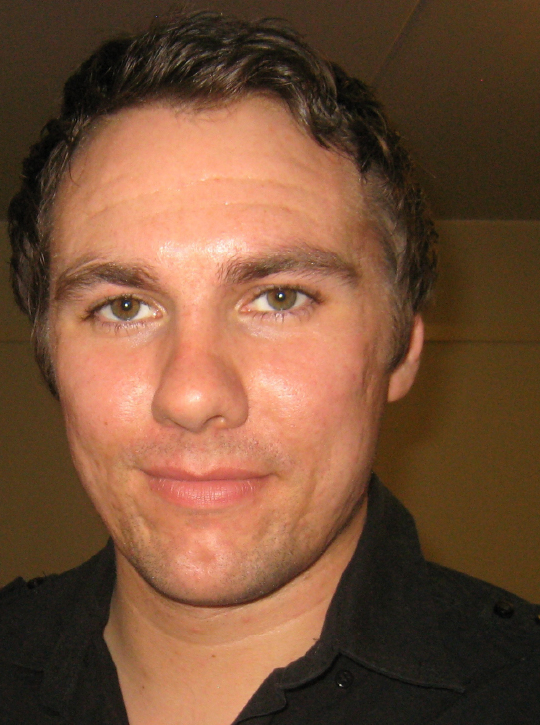
\includegraphics[scale=0.23]{profil} 
    \vspace*{-3em} 
\end{wrapfigure}

\PersonalEntry{}{}
\PersonalEntry{Født}{23.07.1985}
\PersonalEntry{Sivilstatus}{Ugift}
\PersonalEntry{Adresse}{Moldegata 15 H0702, 0445 Oslo}
\PersonalEntry{Telefon}{47057184}
\PersonalEntry{Mail} {\href{mailto:nilspk@ifi.uio.no}{\tt{nilspk@ifi.uio.no}}}
\PersonalEntry{Linkedin}
{\href{http://lnkd.in/JD8kz5}{\tt{http://lnkd.in/JD8kz5}}}
\PersonalEntry{Github}{\href{http://github.com/nilspk}{\tt{github.com/nilspk}}}
\sepspace
% \noindent Jeg er en 26 år gammel student som går bachelor i informatikk på
% UiO, samtidig som jeg jobber deltid som kontormedarbeider hos Kredinor.

% dirty, but works
\section*{Utdanning}
\EducationEntry
{Master i Informatikk, Distribuerte systemer}
{2012$\rightarrow$}
{UiO}
{Jeg studerer nå master, med spesialisering i distribuerte systemer.
Masteroppgaven min går ut på å implementere og evaluere
publish-subscribe systemer for peer-to-peer nettverk.}
\sepspace
\sepspace

\EducationEntry
{Bachelor i Informatikk}
{2009$\rightarrow$2012}
{UiO}
{Fullført bachelor i informatikk: programmering og nettverk våren 2012.
Hvilke fag jeg har tatt i løpet av bacheloren er listet opp på min
Linkedin-profil.}
\sepspace
\sepspace

\EducationEntry
{Ettårig, Nyere Historie}
{2007-08}
{NTNU}
{Ettårig studie i Trondheim med fag som Stormaktspolitikk, Historiefag
og Ex.Phil.}
\sepspace
\sepspace

\EducationEntry
{Forkurs for ingeniørfag}
{2006-07}
{HIST}
{Ettårig utdanning jeg tok for å få den nødvendige fordypningen i Matte,
Fysikk og Kjemi som er påkrevd for å søke mer tekniske studiretninger.}
\sepspace
\sepspace

\EducationEntry
{Videregående utdanning}
{2001 - 2004}
{Ringsaker Videregående}
{Jeg studerte 2 år Medier og Kommunikasjon på Ankerskogen VGS på Hamar,
 hvor vi drev mye med prosjektarbeid,
før jeg tok Allmennfaglig påbygning på Ringsaker VGS.}
\sepspace
\sepspace

\newpage
\section*{Jobberfaring}
\WorkEntry
{Juniorutvikler}
{2012$\rightarrow$}
{Mynt Betalingsterminaler AS}
{Etter å ha jobbet her sommeren 2012 hvor vi utviklet et nytt
brukergrensesnitt som skal brukes på kortterminaler, er dette nå min
faste deltidsjobb. Dette gir meg relevant og praktisk erfaring jeg veldig god
nytte av ved siden av studiene.}
\sepspace
\sepspace

\WorkEntry
{Kontormedarbeider}
{2009 - 2012}
{Kredinor}
{Deltidsansatt på kveldsteam hos Kredinor. Dette er en jobb jeg har hatt
ved siden av studiene i Informatikk. Jeg har jobbet 10 timer i uken
fordelt på to kvelder på hverdager. Å balansere krevende skolearbeid med
deltidsjobb har vært en nyttig og lærerik erfaring.}
\sepspace
\sepspace

\WorkEntry
{Lagermedarbeider}
{2005-08}
{ASKO Hedmark}
{Jobbet som plukker på grossistlager. Dette var en jobb jeg hadde fast
som sommerjobb over noen år, samt en periode på høsten 2008 hvor jeg var
fast ansatt. }
\sepspace

\sepspace
\section*{Kompetanse}
\SkillsEntry{Språk}{Norsk (morsmål)}
\SkillsEntry{}{Engelsk (flytende)}
\sepspace
\SkillsEntry{Programmering}{Java, C, Objective-C, Python, Scheme, SQL, \LaTeX}
\sepspace
\SkillsEntry{OS}{Windows, Mac OS X, Linux}
\sepspace
\SkillsEntry{Annet}{Git, Vim, zsh, screen/tmux,  Arduino, Adobe CS, Eclipse}

\sepspace
\sepspace
\section*{Sideprosjekter}
\WorkEntry
{B.L.I.M.P}
{2011$\rightarrow$}
{En selvflyvende robot!}
{Dette var et prosjekt vi i utgangspunktet startet med i bruksorentert
design, men som var så spennende at vi tok det videre og presenterte det
på Idéfestivalen på Blinderen i September 2011. Video av dette kan sees
her: \href{http://www.bit.ly/ifiblimp}{\tt{youtube-video}}. Prosjektet
har vært ekstremt lærerikt, og planene framover er å ha med roboten vår
på The Gathering, hvor vi har tenkt å promotere instituttet for
Informatikk.}

\sepspace
\sepspace
\section*{Referanse}
% \ReferenceEntry
% {Roger Antonsen}
% {\textit{tlf:}22852482}
% {Førstelektor, Institutt for informatikk}
% {}
% \ReferenceEntry
% {Lise Nordstrøm}
% {\textit{tlf:}90503009}
% {Avdelingsleder, Kredinor}
% {}
Oppgis ved behov.
\end{document}
